\documentclass[border=12pt]{standalone}
\usepackage{tikz}
\usetikzlibrary{arrows.meta, positioning, calc, fit, backgrounds, decorations.pathreplacing}
\usepackage{amsmath, amssymb}

\begin{document}
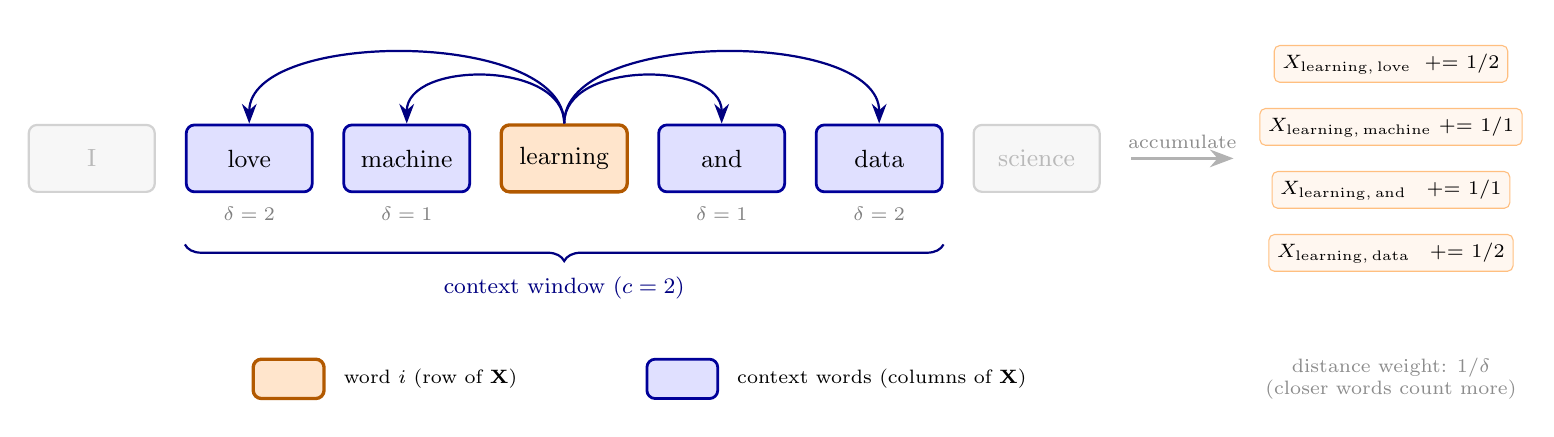
\begin{tikzpicture}[
    word/.style = {rectangle, draw=gray!50, thick, rounded corners=3pt,
                   minimum height=0.85cm, minimum width=1.6cm,
                   font=\small, inner sep=4pt},
    target/.style = {word, draw=orange!70!black, fill=orange!20, line width=1.2pt},
    context/.style = {word, draw=blue!60!black, fill=blue!12, line width=1.0pt},
    outside/.style = {word, fill=gray!6, draw=gray!35, text=gray!55},
    arr/.style = {-{Stealth[length=2.5mm]}, thick, blue!50!black},
    brace/.style = {decorate, decoration={brace, amplitude=6pt, mirror}, thick, blue!50!black},
    countbox/.style = {rectangle, draw=orange!50, fill=orange!6, rounded corners=2pt,
                       font=\scriptsize, inner sep=3pt, minimum width=2.8cm, align=left},
]

%% ---- Sentence words ----
\node[outside]  (w1) at (0, 0)    {I};
\node[context]  (w2) at (2, 0)    {love};
\node[context]  (w3) at (4, 0)    {machine};
\node[target]   (w4) at (6, 0)    {learning};
\node[context]  (w5) at (8, 0)    {and};
\node[context]  (w6) at (10, 0)   {data};
\node[outside]  (w7) at (12, 0)   {science};

%% ---- Window brace ----
\draw[brace] ([yshift=-0.65cm]w2.south west) -- ([yshift=-0.65cm]w6.south east)
    node[midway, below=8pt, font=\footnotesize, blue!50!black] {context window ($c = 2$)};

%% ---- Distance annotations (below word boxes, above the brace) ----
\node[font=\scriptsize, text=black!50] at (2, -0.7) {$\delta=2$};
\node[font=\scriptsize, text=black!50] at (4, -0.7) {$\delta=1$};
\node[font=\scriptsize, text=black!50] at (8, -0.7) {$\delta=1$};
\node[font=\scriptsize, text=black!50] at (10, -0.7) {$\delta=2$};

%% ---- Count arrows from target to context ----
\draw[arr] (w4.north) .. controls +(0, 1.2) and +(0, 1.2) .. (w2.north);
\draw[arr] (w4.north) .. controls +(0, 0.8) and +(0, 0.8) .. (w3.north);
\draw[arr] (w4.north) .. controls +(0, 0.8) and +(0, 0.8) .. (w5.north);
\draw[arr] (w4.north) .. controls +(0, 1.2) and +(0, 1.2) .. (w6.north);

%% ---- Co-occurrence matrix updates (right side) ----
\node[countbox] (c1) at (16.5, 1.2)
    {$X_{\text{learning},\,\text{love}}\;$ += $1/2$};
\node[countbox] (c2) at (16.5, 0.4)
    {$X_{\text{learning},\,\text{machine}}$ += $1/1$};
\node[countbox] (c3) at (16.5, -0.4)
    {$X_{\text{learning},\,\text{and}}\;\;$ += $1/1$};
\node[countbox] (c4) at (16.5, -1.2)
    {$X_{\text{learning},\,\text{data}}\;\;$ += $1/2$};

%% ---- Arrow from window to updates (clear of "science") ----
\draw[-{Stealth[length=3mm]}, thick, gray!60]
    (13.2, 0) -- (14.5, 0)
    node[midway, above, font=\scriptsize, black!45] {accumulate};

%% ---- Legend ----
\node[target, minimum width=0.9cm, minimum height=0.5cm, font=\scriptsize]
    (leg1) at (2.5, -2.8) {};
\node[font=\scriptsize, right=3pt of leg1] {word $i$ (row of $\mathbf{X}$)};

\node[context, minimum width=0.9cm, minimum height=0.5cm, font=\scriptsize]
    (leg2) at (7.5, -2.8) {};
\node[font=\scriptsize, right=3pt of leg2] {context words (columns of $\mathbf{X}$)};

%% ---- Note about distance weighting ----
\node[font=\scriptsize, text=black!45, align=center] at (16.5, -2.8)
    {distance weight: $1/\delta$\\(closer words count more)};

\end{tikzpicture}
\end{document}
